\documentclass[a4paper]{report}

%====================== PACKAGES ======================

\usepackage[english]{babel}
\usepackage[utf8x]{inputenc}
%pour gérer les positionnement d'images
\usepackage{float}
\usepackage{amsmath}
\usepackage{graphicx}
\usepackage{pdfpages}
\usepackage[colorinlistoftodos]{todonotes}
\usepackage{url}
%pour les informations sur un document compilé en PDF et les liens externes / internes
\usepackage{hyperref}
%pour la mise en page des tableaux
\usepackage{array}
\usepackage{tabularx}
%pour utiliser \floatbarrier
%\usepackage{placeins}
%\usepackage{floatrow}
%espacement entre les lignes
\usepackage{setspace}
%modifier la mise en page de l'abstract
\usepackage{abstract}
%police et mise en page (marges) du document
\usepackage[T1]{fontenc}
\usepackage[top=2cm, bottom=2cm, left=2cm, right=2cm]{geometry}
%Pour les galerie d'images
\usepackage{subfig}
%Pour les codes sources
\usepackage{listings}

%====================== INFORMATION ET REGLES ======================

%rajouter les numérotation pour les \paragraphe et \subparagraphe
\setcounter{secnumdepth}{4}
\setcounter{tocdepth}{4}

\hypersetup{							% Information sur le document
pdfauthor = {Simon CHANU},			% Auteurs
pdftitle = {Shepherd Report},			% Titre du document
pdfsubject = {},		% Sujet
%pdfkeywords = {Tag1, Tag2, Tag3, ...},	% Mots-clefs
pdfstartview={FitH}}					% ajuste la page à la largueur de l'écran
%pdfcreator = {MikTeX},% Logiciel qui a crée le document
%pdfproducer = {}} % Société avec produit le logiciel

%======================== DEBUT DU DOCUMENT ========================

\begin{document}

%régler l'espacement entre les lignes
\newcommand{\HRule}{\rule{\linewidth}{0.5mm}}

%page de garde
\begin{titlepage}
    \title{ \normalsize \textsc{Project Report} 
    		\\ [0.5cm]
            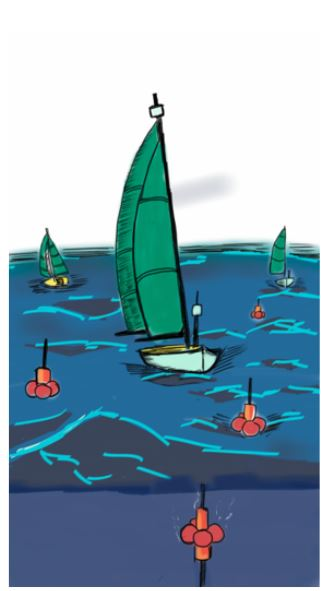
\includegraphics[scale=0.6]{image/logo_SHEPHERD.JPG} % Ou autre image
            \\ [0.3cm]
            \HRule{} 
            \\ [0.5cm]
            \LARGE \textbf{\uppercase{SHEPHERD Project}} 
            \\ [0.20cm]
            \HRule{} 
            \\ [1.0cm]
            
\includegraphics[scale=0.6]{image/logo_ENSTA.jpg}
            %\\
            %\textsc{\textbf{ENSTA Bretagne}}
            \\ [0.5cm]
            \normalsize \today \vspace*{0\baselineskip}
    }

    \date{}
    
    \author{
            \textbf{Students}\\
            \textsc{El Jawad.A,  Chanu.S, Sola.G, Welte.A, Soulie.C, Benet.P, Mehdi.N, } \\
            \textsc{Galland.A, Barronier.R, El Abdalaoui.Z, Finand.C, Zhu.L, Pertierre.S, } \\
            \textsc{Ennouhi.F, Bernardes.E, Tanguy.F} \\
            \\
            \textbf{Supervisor}\\
            \textsc{Luc Jaulin, ENSTA Bretagne} 
    }

    \maketitle
\end{titlepage}

%page blanche
%\newpage
~
%ne pas numéroter cette page
\thispagestyle{empty}
\newpage

% Abstract
\begin{abstract}

	\footnote{Author : Simon CHANU} The SHEPHERD Project aims to command a swarm of robotic oceanographic buoys by the astute use of the different directions of the current at along the water column, with the help of an acoustic localization system provided by robotic sailboats acting as shepherds. This paper describes the simulation created to validate the foundations of the project. This simulation uses simple models and equations to effectively command a swarm of robots.

\end{abstract}

\tableofcontents
%ne pas numéroter le sommaire

\newpage

\listoffigures
\thispagestyle{empty}
\setcounter{page}{0}

\newpage

%espacement entre les lignes d'un tableau
\renewcommand{\arraystretch}{1.5}

%====================== INCLUSION DES PARTIES ======================

~
\thispagestyle{empty}
%recommencer la numérotation des pages à "1"
\setcounter{page}{0}
\newpage

\chapter{Presentation of the Shepherd project}
\section{Given issue}
\section{Our solution}
\section{TDOA method}
\subsection{Introduction}
\footnote{Section written by E. Bernardes and S. Pertierre} 
In our settings we have four boats that should simultaneously send signals to the buoy, informing their positions (known due to each boat's GPS system) and time of emission (each boat has also an internal clock, considered to be synchronized). 
%
The buoys have to be programmed in a way that make it possible for them to receive these data and calculate their position. 

One possible way to solve this problem is to put a clock inside each buoy.% make it send a back signal to the boats. 
%
In this way, using the fact that we know the signal's velocity in the sea, we can easily calculate the distances of the buoy to each one of the boats by doing the following calculation:
\begin{equation}
d_n = ||p - q_n|| = c(t_n - t_0)
\label{eq:distance}
\end{equation}
Where $d_n$ is the distance of the buoy to the $n$th boat, $q_n = (q_{nx},q_{ny},q_{nz})$ is the position of said boat, $p = (p_x,p_y,p_z)$ is the buoy's position in the sea, $c$ is the signal's velocity in the medium, $t_0$ is the time of emission and $t_n$ is the time when the buoy receive the $n$th boat's signal. 
%
We can calculate all distances in this way and then triangulate the buoy's position.

It is indeed a simple and efficient method of calculation. Nevertheless, it can be difficult to guarantee that the buoy's internal clock is well synchronized with those of the boats, raising the possibility of high uncertainties in the calculations.
%
It is not impossible to do so, but the needed precision clock can be expensive. The Time Difference of Arrival (TDOA) method is proposed to replace this method of calculation and overcome this difficulty.
%
% TODO: INSERT BOATS AND BUOY FIGURE
% \label{fig:boats_buoy_signals}
\subsection{Method principle}
The method consists in substituting the buoy's clock by??? a chronometer.
%
The chronometer is not capable of knowing the exact moments of the signals arrivals, but it is able to keep track of the time difference between each signal.

When the buoy receives the first boat's signal, if launches the chronometer and waits for the arrival of the other signals, keeping track of the time between then.
%
They buoy stores then the values $\tau_2 = t_2 - t_1$, $\tau_3 = t_3 - t_1$ and $\tau_4 = t_4 - t_1$; as shown in the Figure \ref{fig:time_differences}.
%
% TODO: INSERT TIME DIFFERENCES FIGURE
% \label{fig:time_differences}
The equation \ref{eq:distance} is still valid, and applying it to our project, we have the system of linear equations described in \ref{eq:distance_system}.
\begin{align}
d_1 = ||p - q_1|| &= c(t_1 - t_0) \nonumber \\
d_2 = ||p - q_2|| &= c(t_2 - t_0) \\
d_3 = ||p - q_3|| &= c(t_3 - t_0) \nonumber \\
d_4 = ||p - q_4|| &= c(t_4 - t_0) \nonumber 
\label{eq:distance_system}
\end{align}

Substituting the time differences $\tau_n$ in \ref{eq:distance_system}, we have the following final system:
\begin{align}
||p - q_1|| &= c(t_1 - t_0) \nonumber \\
||p - q_2|| &= c(t_1 + \tau_2 - t_0) \\
||p - q_3|| &= c(t_1 + \tau_3 - t_0) \nonumber \\
||p - q_4|| &= c(t_1 + \tau_4 - t_0) \nonumber 
\label{eq:distance_tdoa}
\end{align}
Since $q_n$, $c$, $t_0$ and $\tau_n$ are all known, then the only unknowns in the system are $t_1$, $p_x$, $p_y$ and $p_z$. Since we have 4 equations and 4 unknowns, we can easily solve this system to find the $p$ vector.
%
Since the buoy's are also equipped with ballasts, we also known the value $p_z$ in our case, our number of equations is bigger than our number of unknown variables.


\chapter{Team management methods}
\section{Scrum}
\section{Github}

\chapter{Simulation theory}
\section{Simulation of the environment}
\section{Simulation of the sailboats}
\section{Simulation of the buoys}

\chapter{Simulation architecture}
\section{ROS presentation}
\section{ROS architecture}
    
\chapter{Display}
\section{OpenGL}
\subsection{presentation}

Open Graphics Library (OpenGL) is a cross-language, cross-platform application programming interface (API) for rendering 2D and 3D vector graphics. The API is typically used to interact with a graphics processing unit (GPU), to achieve hardware-accelerated rendering.

We chose to use OpenGl 1.1 as a soft and reliable 3d rendering system. OpenGl is a low level rendering library. Unlike high level graphic engine such as Unity, it is easy to print vector fields and soft graphic that are easy to see. With realistic graphics, it can be difficult to see the data between the reflects of the light and the real opacity of watter for example. With Opengl, transparency of watter can be adjusted for a better visualisation.

OpenGl does not work alone. It has to be integrated in the window manager of the operating system. An open source library SDL (Simple Direct media Layer) enables to use the graphic interface of most of the operating systems. Moreover, it provides keyboards and mouse support so that the user can navigate in the 3d environnement and interact with the window. SDL provides also a lot of features such as sound handling and other device support.
 
\subsection{3d features}

The 3d geometric object that we print are the sea, the boats, the buoys, the vector fields, the grid pattern and the localisations of the intervals. The sea is made of two layer of transparent blue sqares, so that looking to the sea from the outside looks darker that from the inside. And everything that is in the sea looks blue. The boats geometry have been recovered from an older sailboat control simulation. The veil and rudder are movable. The buoys are simple red spheres.


\subsection{camera control}

The camera control system is a first person view. The camera can be controlled in the six local axis of the view (three rotations and three translations) thanks to the mouse. This enables a practical and intuitive navigation in all directions.

The mouse wheel enables to move forward and backward. holding the left mouse button of the camera while moving the mouse moves the scene perpendicularly to the camera. holding the right mouse button while moving the mouse rotates the camera on an axis perpendicular to the camera axis. holding both right and left button enables to rotate the camera on its axis.

Camera handling is often used by an extern 3 by 3 matrix system that has to be implemented. However, this time, only the OpenGl transformation system has been used to control the camera. OpenGl possessed its own matrix 4 by 4 stack that includes rotation and translation and also includes multiplication function and generation of basic matrix such as rotation and translation matrix. The purpose of this matrix stack is to apply successive affine transformation to the geometry. But we can use it as a computationnal tool. OpenGl provides a function to store in our program the current transformation matrix. So to compute matrix multiplication and rotation matrix generation, we will store the current matrix transformation in a variable; load the matrix we want on the opengl matrix stack; compute transformations; get the result in an other variable; put back the initial transformation result so that opengl has seen nothing. 

\section{Unity3D}
\subsection{Presentation}

% IMAGE: Logo Unity

Unity3D is a game engine developed by Unity Technologies. It is widely used in the developpment of video games, especialy on mobile devices and websites because it is one of the more lightweight game engine available. It uses the aforementioned OpenGL API to use the processing power of the machine it is installed on. It also provided an abstraction level allowing the programmer to easily add 3D Objects in a scene, manage lighting option, texture and many other functionalities. Unity also offers a physics engine that can compute collision, gravity as well as more complicated patterns such as moving cloth and water. 

In our project we use Unity as a graphical engine, we choose not to use the physic engine in order to have complete control over the behaviours of the sailboats and buoys. The simulation program computes the state of the world, this is then send to Unity that displays the new state of the world. Because Unity is intended to be used more as a pleasing graphical tool than a exact representation of the simulation, liberties may be taken on the position of the objects in order to obtain smoother movement.

\subsection{Communication with the simulation}
\subsubsection{Server-Client link}

To comunicate between the simulation and Unity, a client-server architecture has been choosen. This choice has servral advantages:
\begin{itemize}
\item A modular architecture: enabling the two programs to work independantly and making the development of the programs easier to split into two separate teams.
\item An online architecture: enabling the programs to run on a same machine or on distant machines
\item A language agnostic architecture: enabling the simulation and the display to use different languages (C++ for the simulation, C\# for Unity)
\end{itemize}

\subsubsection{JSON format}

To communicate data, JSON parsing is used. This method format variables (test, numbers, etc) into a text that contains all the variables and that can be easily extracted by Unity. JSON was introduced by Javascript but librairies are know available on most mainstream languages making it an ideal solution to communicate data between two languages

\lstset{
    string=[s]{"}{"},
    stringstyle=\color{blue},
    comment=[l]{:},
    commentstyle=\color{black},
}
\renewcommand{\lstlistingname}{Code}
\begin{lstlisting}[caption=JSON format, frame=single]
{
    "Sailboat":
    {
        "name":"Auv0",
        "sailYaw":-13.1802,
        "x":-19.2049,
        "y":20.338,
        "yaw":-296.908
    }
}
\end{lstlisting}

This formating made it esay to add a the buoys later in the project. % TODO

\subsection{Unity Objects}
\subsubsection{Graphical Objects}

% IMAGE: d'un objet

\subsubsection{SimulationManager}

SimulationManager is the main object of the scene. It has two scripts TCPServer.cs and SimulationManager.cs that provide communication with the simulation and dynamically instanciate the objects (sailboats and buoys). 

TCPServer.cs is the implementation of the client-server architecture. It listens to the simulation and record a stream of one or sevral JSON strings. This stream is then processed to extract individual JSON string that are then send to SimulationManager.cs.

SimulationManager.cs extract the data of the messages from TCPServer.cs and either create a new object if the message corespond to a new object or update the state of an existing entity. % TODO

\subsection{Results}

% IMAGE

% ===================== Conclusion ====================
\newpage

	\begin{center}
		\textbf{\LARGE{Conclusion}}
	\end{center}

\vspace{5cm}

Conclusion

\newpage
%récupérer les citation avec "/footnotemark"
\nocite{*}

% ====================== Biblio ======================

%choix du style de la biblio
\bibliographystyle{plain}
%inclusion de la biblio
\bibliography{Rapport2A}
%voir wiki pour plus d'information sur la syntaxe des entrées d'une bibliographie


% ====================== Annexes ======================
\newpage

	\begin{center}
		\title{ \HRule{} \\ [12cm]
				\LARGE \textbf{\uppercase{Annexes}}\\ [12cm]
				\HRule{}}
		\maketitle
	\end{center}

\end{document}
